\documentclass{beamer}

\usefonttheme{serif}
\usepackage{dsfont}
\setbeamersize{text margin left=5pt, text margin right=5pt}

\newcommand{\bgk}[1]{\boldsymbol{#1}}

\newcommand{\bzero}{\bgk{0}}
\newcommand{\bone}{\bgk{1}}

\newcommand{\balpha}{\bgk{\alpha}}
\newcommand{\bnu}{\bgk{\nu}}
\newcommand{\bbeta}{\bgk{\beta}}
\newcommand{\bxi}{\bgk{\xi}}
\newcommand{\bgamma}{\bgk{\gamma}} 
\newcommand{\bo}{\bgk{o }}
\newcommand{\bdelta}{\bgk{\delta}}
\newcommand{\bpi}{\bgk{\pi}}
\newcommand{\bepsilon}{\bgk{\epsilon}} 
\newcommand{\bvarepsilon}{\bgk{\varepsilon}} 
\newcommand{\brho}{\bgk{\rho}}
\newcommand{\bvarrho}{\bgk{\varrho}}
\newcommand{\bzeta}{\bgk{\zeta}}
\newcommand{\bsigma}{\bgk{\sigma}}
\newcommand{\boldeta}{\bgk{\eta}}
\newcommand{\btay}{\bgk{\tau}}
\newcommand{\btheta}{\bgk{\theta}}
\newcommand{\bvertheta}{\bgk{\vartheta}}
\newcommand{\bupsilon}{\bgk{\upsilon}}
\newcommand{\biota}{\bgk{\iota}}
\newcommand{\bphi}{\bgk{\phi}}
\newcommand{\bvarphi}{\bgk{\varphi}}
\newcommand{\bkappa}{\bgk{\kappa}}
\newcommand{\bchi}{\bgk{\chi}}
\newcommand{\blambda}{\bgk{\lambda}}
\newcommand{\bpsi}{\bgk{\psi}}
\newcommand{\bmu}{\bgk{\mu}}
\newcommand{\bomega}{\bgk{\omega}}

\newcommand{\bA}{\bgk{A}}
\newcommand{\bDelta}{\bgk{\Delta}}
\newcommand{\bLambda}{\bgk{\Lambda}}

\newcommand{\bvec}[1]{\mathbf{#1}}

\newcommand{\va}{\bvec{a}}
\newcommand{\vb}{\bvec{b}}
\newcommand{\vc}{\bvec{c}}
\newcommand{\vd}{\bvec{d}}
\newcommand{\ve}{\bvec{e}}
\newcommand{\vf}{\bvec{f}}
\newcommand{\vh}{\bvec{h}}
\newcommand{\vi}{\bvec{i}}
\newcommand{\vj}{\bvec{j}}
\newcommand{\vk}{\bvec{k}}
\newcommand{\vl}{\bvec{l}}
\newcommand{\vm}{\bvec{m}}
\newcommand{\vn}{\bvec{n}}
\newcommand{\vo}{\bvec{o}}
\newcommand{\vp}{\bvec{p}}
\newcommand{\vq}{\bvec{q}}
\newcommand{\vr}{\bvec{r}}
\newcommand{\vs}{\bvec{s}}
\newcommand{\vt}{\bvec{t}}
\newcommand{\vu}{\bvec{u}}
\newcommand{\vv}{\bvec{v}}
\newcommand{\vw}{\bvec{w}}
\newcommand{\vx}{\bvec{x}}
\newcommand{\vy}{\bvec{y}}
\newcommand{\vz}{\bvec{z}}

\newcommand{\vA}{\bvec{A}}
\newcommand{\vB}{\bvec{B}}
\newcommand{\vC}{\bvec{C}}
\newcommand{\vD}{\bvec{D}}
\newcommand{\vE}{\bvec{E}}
\newcommand{\vF}{\bvec{F}}
\newcommand{\vH}{\bvec{H}}
\newcommand{\vI}{\bvec{I}}
\newcommand{\vJ}{\bvec{J}}
\newcommand{\vK}{\bvec{K}}
\newcommand{\vL}{\bvec{L}}
\newcommand{\vM}{\bvec{M}}
\newcommand{\vN}{\bvec{N}}
\newcommand{\vO}{\bvec{O}}
\newcommand{\vP}{\bvec{P}}
\newcommand{\vQ}{\bvec{Q}}
\newcommand{\vR}{\bvec{R}}
\newcommand{\vS}{\bvec{S}}
\newcommand{\vT}{\bvec{T}}
\newcommand{\vU}{\bvec{U}}
\newcommand{\vV}{\bvec{V}}
\newcommand{\vW}{\bvec{W}}
\newcommand{\vX}{\bvec{X}}
\newcommand{\vY}{\bvec{Y}}
\newcommand{\vZ}{\bvec{Z}}

\usepackage{subcaption}

\usepackage{xcolor}
\usepackage[utf8]{inputenc}
\DeclareFontEncoding{LS1}{}{}
\DeclareFontSubstitution{LS1}{stix}{m}{n}
\DeclareSymbolFont{symbols2}{LS1}{stixfrak} {m} {n}
\DeclareMathSymbol{\operp}{\mathbin}{symbols2}{"A8}
\setbeamertemplate{navigation symbols}{}

\usepackage{lipsum}

\newcommand\blfootnote[1]{%
  \begingroup
  \renewcommand\thefootnote{}\footnote{#1}%
  \addtocounter{footnote}{-1}%
  \endgroup
}

\addtobeamertemplate{navigation symbols}{}{%
    \usebeamerfont{footline}%
    \usebeamercolor[fg]{footline}%
    \hspace{1em}%
    \insertframenumber/\inserttotalframenumber
}

\title{
Randomized Numerical Linear Algebra\\
Lecture 1
}
%\subtitle{Mathematical framework, existence and exactness}

\author{F. M. Faulstich}
\date{01/09/2024}


\begin{document}

\frame{\titlepage}

\begin{frame}{}
    
\end{frame}


\begin{frame}{Planned course Outlook}

\begin{enumerate}
    \item Review of numerical linear algebra and probability theory
    \item Trace estimation and Schatten $p$-norm estimation (M.C. methods)
    \item Sampling to approximate matrices (matrix multiplication)
    \item Randomized linear embedding
    \item Randomized techniques to find subspace
that is aligned with the range of a matrix 
    \item Randomized algorithms for computing matrix factorizations
    \item Solving linear systems with randomized techniques
\end{enumerate}

\end{frame}

\begin{frame}{What to expect!}

\begin{itemize}
    \item[$\bullet$] The course is centered primarily on computational aspects
    \item[$\bullet$] Aimed at equipping you with a robust set of computational skills
    \item[$\bullet$] Proofs will be included occasionally, but only at a high level
    \item[$\bullet$] The course aims to impart an understanding of the key ideas behind proofs rather than delving into exhaustive, fully worked-out proofs
\end{itemize}

\end{frame}

\begin{frame}{numerical linear algebra}

\begin{itemize}
    \item[$\bullet$]<1-> solving dense and sparse linear systems
    \item[$\bullet$]<2-> orthogonalization, least square \& Tikhonov regularization
    \item[$\bullet$]<5-> determination of eigenvalues \& eigenvectors, invariant subspaces
    \item[$\bullet$]<7-> singular value decomposition (SVD)
\end{itemize}    
\only<1>{\centering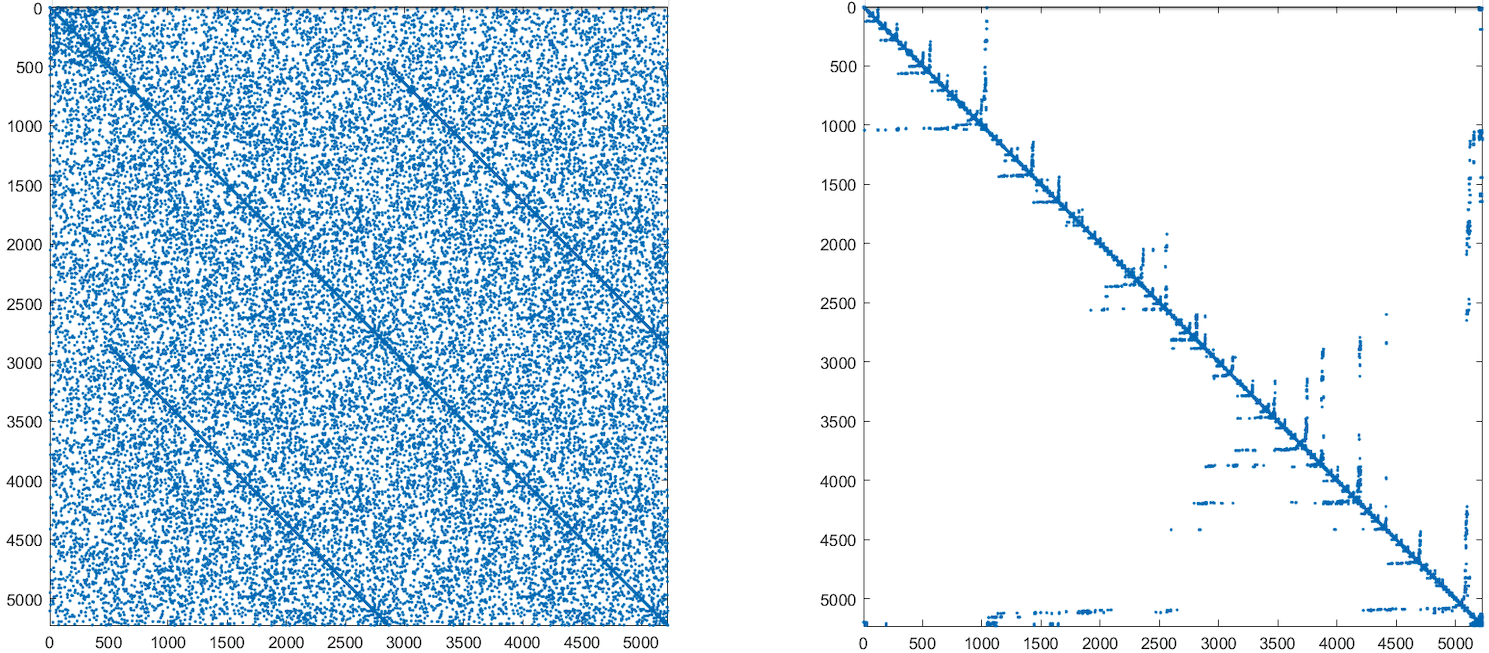
\includegraphics[width = 0.5\textwidth]{Graphics/Screenshot 2024-01-07 at 2.21.58 PM.png}
}

\only<2>{\centering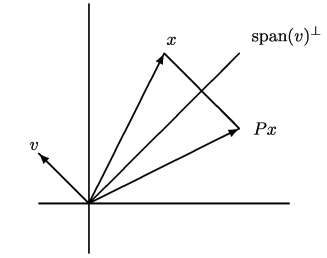
\includegraphics[width = 0.4\textwidth]{Graphics/Screenshot 2024-01-07 at 2.25.59 PM.png}
}

\only<3>{\centering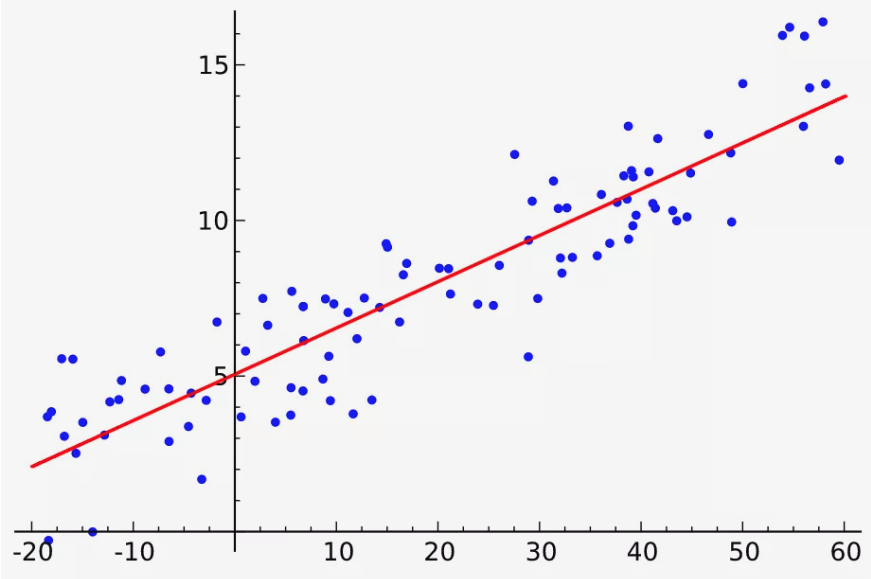
\includegraphics[width = 0.4\textwidth]{Graphics/Screenshot 2024-01-07 at 2.39.05 PM.png}
} 

\only<4>{\centering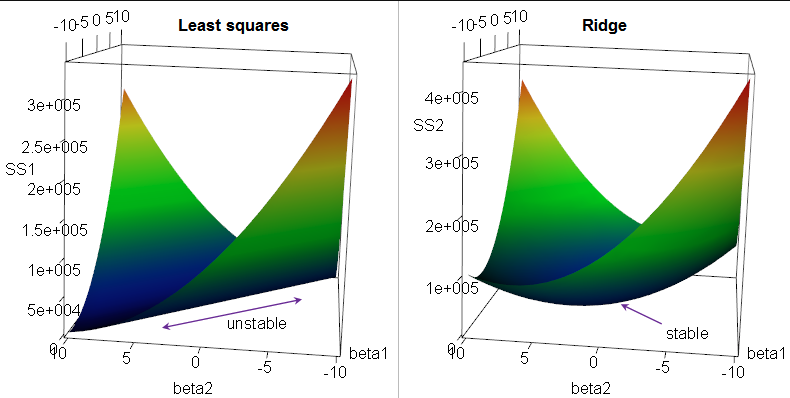
\includegraphics[width = 0.6\textwidth]{Graphics/Screenshot 2024-01-07 at 2.43.44 PM.png}
} 

\only<5>{\centering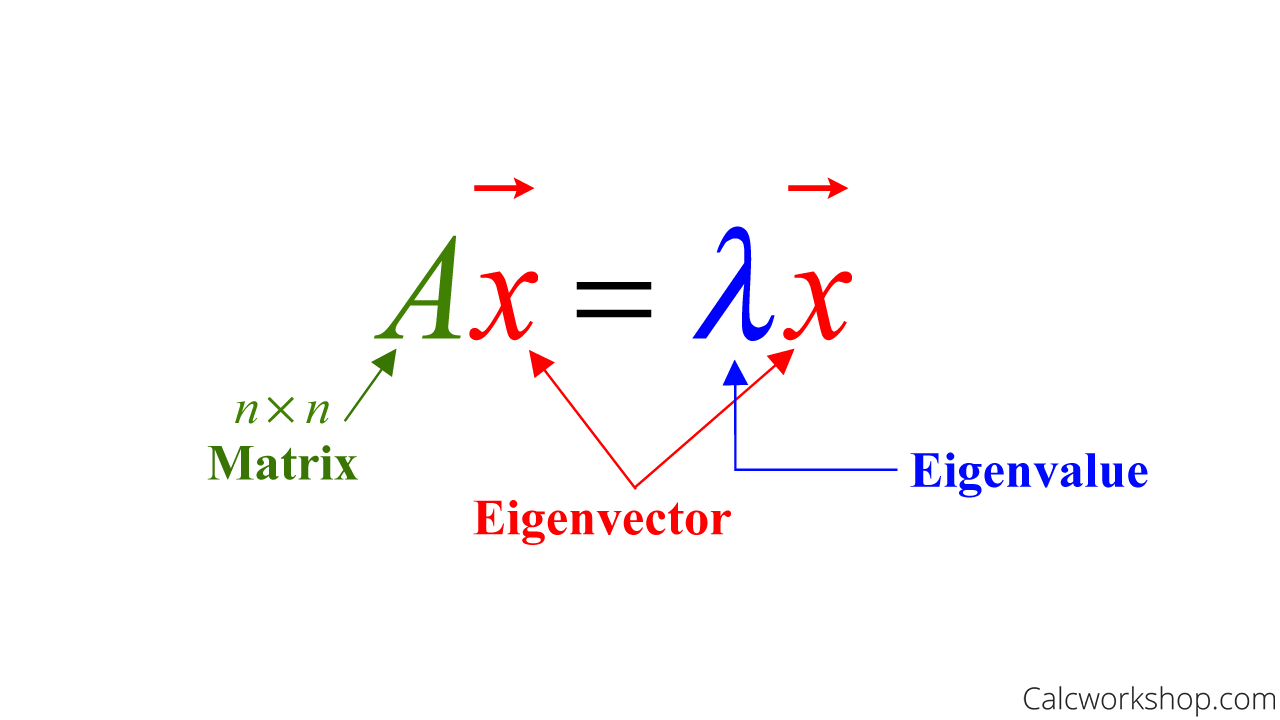
\includegraphics[width = 0.6\textwidth]{Graphics/eigenvalue-eigenvector-formula-definition.png}
} 

\only<6>{\centering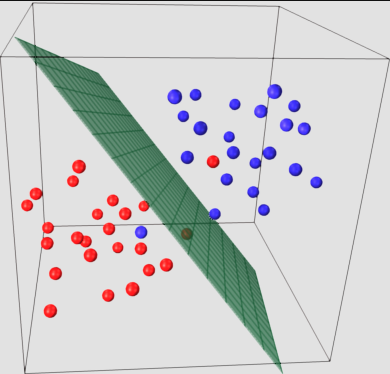
\includegraphics[width = 0.3\textwidth]{Graphics/Screenshot 2024-01-07 at 2.51.18 PM.png}
} 

\only<7>{\centering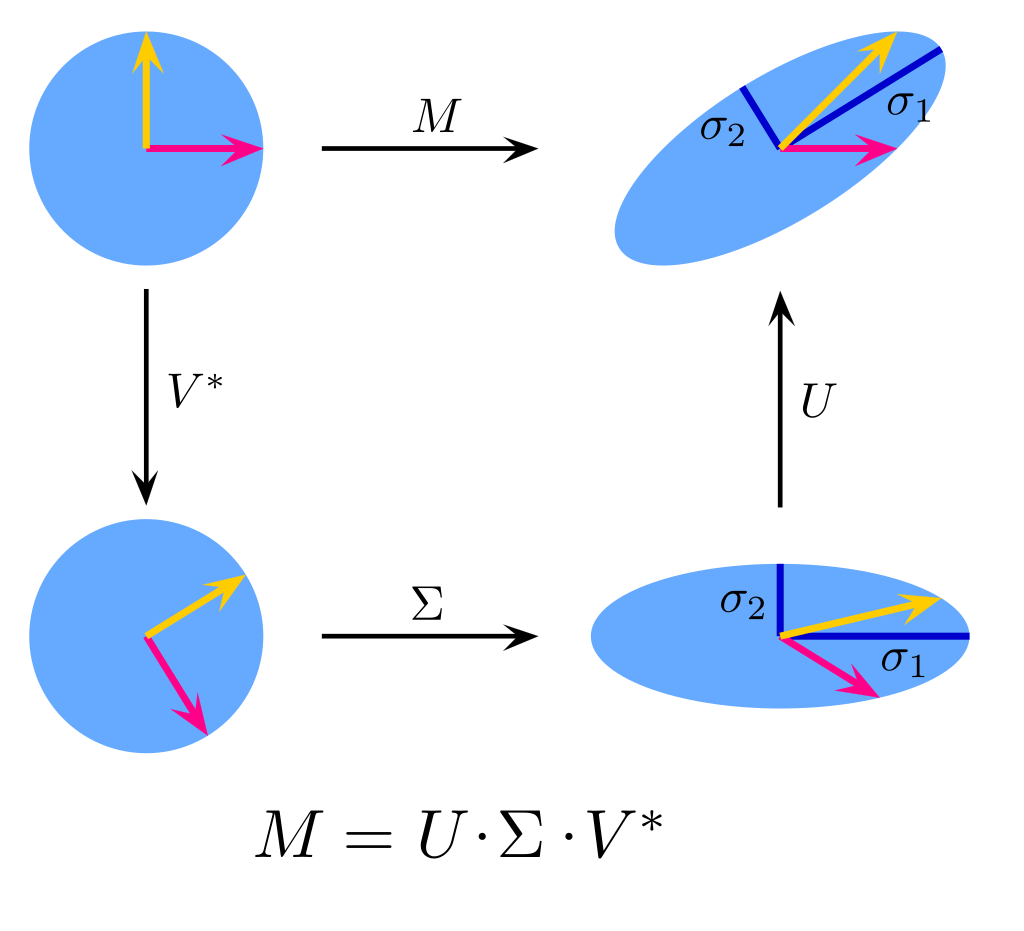
\includegraphics[width = 0.4\textwidth]{Graphics/1024px-Singular-Value-Decomposition.svg.png}
} 

\end{frame}


\begin{frame}{Numerical linear algebra}

What is the problem?\\
~\\
$\Rightarrow$ Large scaling problems!\\
% ~\\
% Example:\\
% Some example
\end{frame}

\begin{frame}{Numerical linear algebra}

\begin{center}
``Randomized'' linear algebra offers novel tools addressing these challenges
\end{center}

\end{frame}


\begin{frame}{Randomized algorithms}
\begin{enumerate}
    \item Monte Carlo (M.C.) algorithms ($\sim$1940)\\
    $\cdot$ Last resort methods\\
    $\cdot$ M.C. converges slowly\\
    $\cdot$ Hesitation: Two runs should produce the same number
    \item Randomized algorithms in numerical linear algebra ($\sim$1980)\\
    $\cdot$ Power method, random initialization (Dixon 1983)\\
    $\cdot$ M.~C.~methods for trace estimation (Girard 1989 \& Hutchinson 1990)\\
    $\cdot$ Randomized transformations can avoid pivoting
steps in Gaussian elimination (Parker 1995)\\
    \item  Practical randomized algorithms for low-rank matrix approximation and least-squares problems (mid-2000s)\\
    $\cdot$ First computational evidence that randomized algorithms outperform classical NLA algorithms for particular classes of problems
\end{enumerate}
\end{frame}


\begin{frame}{}
\vspace{2.5cm}
\begin{center}
\begin{Large}
    Review:\\
    Classical Numerical Linear Algebra
\end{Large}
\end{center}
\vspace{1.5cm} 
\begin{footnotesize}
\begin{itemize}
    \item[$\bullet$] L. N. Trefethen and D. Bau III, Numerical linear algebra, Vol. 50, SIAM
    \item[$\bullet$] G. Stewart, Matrix Algorithms Volume 1: Basic Decompositions, SIAM
    \item[$\bullet$] G. W. Stewart, Matrix algorithms volume 2: eigensystems, Vol. 2, SIAM
    \item[$\bullet$] G. H. Golub and C. F. Van Loan, Matrix computations
    \item[$\bullet$] R. A. Horn and C. R. Johnson, Matrix analysis
    \item[$\bullet$] R. Bhatia, Matrix analysis, Vol. 169 of Graduate Texts in Mathematics
\end{itemize}
\end{footnotesize}

\end{frame}

\begin{frame}{Basics -- Notation I}

\begin{itemize}
    \item[$\bullet$] Algebraic field: 
    $\mathbb{C}$, $\mathbb{R}$, $\mathbb{F}$
    \item[$\bullet$] Scalars: 
    $a,b, ...$ or $\alpha, \beta, ...$
    \item[$\bullet$] Vectors are elements of $\mathbb{F}^n$, $n\in\mathbb{N}$:
    $\va, \vb, ...$ or $\balpha, \bbeta, ...$ 
    \item[$\bullet$] Special vectors $\bzero, \bone, \bdelta_i \in \mathbb{F}^n$:
    $$
    \bzero = \begin{pmatrix} 0\\ 0 \\ \vdots \\ 0 \end{pmatrix}
    \quad
    \bone = \begin{pmatrix} 1\\ 1 \\ \vdots \\ 1 \end{pmatrix}
    \quad
    \bdelta_i = \begin{pmatrix} 0\\ \vdots \\ 0 \\ 1\\ 0 \\ \vdots \\ 0 \end{pmatrix}
    $$
    \item[$\bullet$] Vector element:
    $$
    (\va)_{i} = \va({i}) \qquad i\rm{th\;coordinate\;of\; \va}  
    $$
    \item[$\bullet$] Colon notation: $(\va)_{1:i} = \va(1:i)$
\end{itemize}
\end{frame}


\begin{frame}{Basics -- Notation II}

\begin{itemize}
    \item[$\bullet$] A matrix is an element of $\mathbb{F}^{m\times n}$, $m, n\in\mathbb{N}$:\\
    $\vA, \vB, ...$ or $\bLambda, \bDelta, ...$
    \item[$\bullet$] Matrix element:
    $$
    (\vA)_{ij} = \vA({ij}) \qquad (i,j)\rm{th\;coordinate\;of\; \vA}  
    $$
    \item[$\bullet$] Special matrices $\bzero, \vI \in \mathbb{F}^{m\times n}$:
    $$
    \bzero = 
    \begin{pmatrix}
    0       & \cdots    & 0 \\
    \vdots  & \ddots    & \vdots\\
    0       & \cdots    & 0
    \end{pmatrix}
    \quad
    \vI = 
    \begin{pmatrix}
    1       & 0         & \cdots    & 0 \\
    0       & \ddots    & \ddots    & \vdots\\
    \vdots  & \ddots    &  1        & 0\\
    0       & \cdots    & 0         & 1
    \end{pmatrix}
    $$
    \item[$\bullet$] Colon notation: 
    $(\vA)_{i:}\equiv$ $i$th row and $(\vA)_{:j}$ $j$th column of $\vA$
\end{itemize}
\end{frame}

\begin{frame}{Basics -- Notation III}
\begin{itemize}
    \item[$\bullet$] $*$ is the conjugate transpose
    \item[$\bullet$] $\mathbb{H}_n = \mathbb{H}_n(\mathbb{F}) = \{ \vA\in\mathbb{F}^{n\times n}~:~ \vA = \vA^* \}$
    \item[$\bullet$] $\dagger$ is the Moor--Penrose (pseudo)inverse: 
    $\vA^\dagger$ is the MP inverse of $\vA$ iff
    \begin{equation*}
    \begin{aligned}
    (i)&\quad  ~\vA\vA^\dagger\vA = \vA \qquad &(iii)&\quad  (\vA\vA^\dagger)^* = \vA\vA^\dagger\\
    (ii)&\quad \vA^\dagger\vA\vA^\dagger = \vA^\dagger \qquad &(iv)&\quad (\vA^\dagger\vA)^* = \vA^\dagger\vA
    \end{aligned}
    \end{equation*}
    If $\vA$ has full column rank, then  $\vA^\dagger = (\vA^* \vA)^{-1} \vA^*$\\
    If $\vA$ attains an inverse then
    $$
    \vA^\dagger = \vA^{-1}
    $$
\end{itemize}

\end{frame}

\begin{frame}{Eigenvalues and singular values}

\begin{itemize}
    \item[$\bullet$] PSD$=\{\vA \in \mathbb{H}_n ~:~ \vx^\top \vA \vx \geq 0 ~{\rm for}~ \vx \neq 0\}$
     \item[$\bullet$] \;~PD$=\{\vA \in \mathbb{H}_n ~:~ \vx^\top \vA \vx > 0 ~{\rm for}~ \vx \neq 0 \}$
     \item[$\bullet$] $\preccurlyeq$ denotes the semidefinte order on $\mathbb{H}_n$, i.e. 
     $$
     \vA \preccurlyeq \vB \Leftrightarrow 0 \preccurlyeq \vB- \vA
     $$
     \item[$\bullet$] $\prec$ denotes the semidefinte order on $\mathbb{H}_n$, i.e. 
     $$
     \vA \prec \vB \Leftrightarrow 0  \prec \vB- \vA
     $$
     \item[$\bullet$] Eigenvalues of $\vA\in \mathbb{H}_n$: $\lambda_1 \geq \lambda_2\geq ...$
     \item[$\bullet$] Singular values of $\vA\in\mathbb{F}^{m\times n}$: $\sigma_1 \geq \sigma_2\geq ...$
     \item[$\bullet$] Let $f:\mathbb{R} \to \mathbb{R}$. We extend $f$ to spectral function $f:\mathbb{H}_n \to \mathbb{H}_n$
     $$
     f(\vA)
     :=
     \sum_{i=1}^n f(\lambda_i) \vu_i \vu_i^*
    \quad {\rm where} \quad
    \vA = \sum_{i=1}^n \lambda_i \vu_i \vu_i^*
     $$
\end{itemize}
\end{frame}

\begin{frame}{Inner products and geometry I}

\begin{itemize}
    \item[$\bullet$] Equip $\mathbb{F}^n$ with standard scalar product and associated $\ell^2$-norm.\\
    Let $\va, \vb \in \mathbb{F}^n$ then
    $$\langle \va, \vb  \rangle := \va \cdot \vb = \va^* \vb = \sum_{i=1}^n (\va)_i^* (\vb)_i$$
    and
    $$\Vert \va \Vert^2 := \langle \va, \va  \rangle$$\
    \item[$\bullet$] Unit sphere in $\mathbb{F}^n$: $\mathbb{S}^{n-1} = \mathbb{S}^{n-1}(\mathbb{F})$
\end{itemize}
    
\end{frame}

\begin{frame}{Inner products and geometry II}

\begin{itemize}
    \item[$\bullet$] The trace of $\vA \in \mathbb{F}^{n\times n}$: 
    $$
    {\rm Tr}(\vA) = {\rm trace} (\vA) = \sum_{i=1}^n (\vA)_{ii}
    $$
    Nonlinear functions bind before the trace.
    \item[$\bullet$] Equip $\mathbb{F}^{m\times n}$ with the standard trace inner product and Frobenius norm:\\
    Let $\vA, \vB \in \mathbb{F}^{m \times n}$ then
    $$\langle \vA, \vB  \rangle := {\rm Tr} (\vA^* \vB)$$
    and
    $$
    \Vert \vA \Vert_{F}^2 =  \langle \vA, \vA  \rangle
    $$
    \item[$\bullet$] $\vU \in \mathbb{F}^{m \times n}$ is orthonormal iff $\vU^* \vU = \vI_{n}$.\\ 
    $\vU$ is unitary ($\mathbb{F} = \mathbb{C}$) or orthogonal $(\mathbb{F} = \mathbb{R})$ if $m=n$.  
\end{itemize}
    
\end{frame}

\begin{frame}{Matrix norms I}

\begin{itemize}
\item[$\bullet$] Let $\Vert \cdot \Vert_{\alpha}$ be a norm on $\mathbb{F}^n$ and $\Vert \cdot \Vert_{\beta}$ be a norm on $\mathbb{F}^m$. Then
$$
\Vert \cdot \Vert_{\alpha, \beta}:\mathbb{F}^{m \times n} \to \mathbb{R}
; \vA \mapsto \sup_{\substack{\vx\in\mathbb{F}^n \\ \Vert \vx \Vert_\alpha \neq 0}}
\frac{\Vert \vA \vx \Vert_{\beta}}{\Vert \vx \Vert_\alpha}
$$
Induces a norm on $\mathbb{F}^{m \times n}$.
\item[$\bullet$] Alternatively, we may define any function
$$
\Vert \cdot \Vert : \mathbb{F}^{m \times n} \to \mathbb{R}
$$
that fulfills:
\begin{enumerate}
    \item $0 \leq \Vert \vA \Vert,~ \forall \vA \in \mathbb{F}^{m \times n}$ and $\Vert \vA \Vert = 0  \Leftrightarrow \vA = \bzero$
    \item $\Vert a \vA \Vert = |a| \Vert \vA \Vert,~ \forall \vA \in \mathbb{F}^{m \times n},$ and $\forall a\in\mathbb{F}$
    \item $\Vert \vA + \vB \Vert \leq \Vert \vA \Vert + \Vert \vB \Vert,~\forall \vA, \vB \in \mathbb{F}^{m \times n}$
\end{enumerate}
\item[$\bullet$] $\Vert \cdot \Vert$ is an induced matrix norm iff 
\end{itemize}

\end{frame}

\begin{frame}{Matrix norms II}
Several matrix norms will be used. Let $\vA \in \mathbb{F}^{m \times n}$
\begin{itemize}
    \item[$\bullet$] The unadorned norm $\Vert \cdot \Vert$ is the spectral norm
    $$
    \Vert \vA \Vert 
    =
    \sigma_1
    =
    \Vert \vA \Vert_{\ell^2} 
    $$
    \item[$\bullet$] $\Vert \cdot \Vert_*$ is the nuclear/trace norm
    $$
    \Vert \vA \Vert_*
    =
    \sum_{k=1}^{\min(m,n)} \sigma_k
    $$
    \item[$\bullet$] $\Vert \cdot \Vert_F$ is the Frobenius norm
    $$
    \Vert \vA \Vert_F^2
    =
    \sum_{i=1}^m\sum_{j=1}^n |(A)_{ij}|^2
    =
    \sum_{k=1}^{\min(m,n)} \sigma_k^2
    =
    {\rm Tr}(\vA^* \vA)
    $$
\end{itemize}
\end{frame}

\begin{frame}{Matrix norms III}

\begin{itemize}
    \item[$\bullet$] $\Vert \cdot \Vert_p$ is the Schatten p-norm for $p\in [1,\infty]$
    $$
    \Vert \vA \Vert_p
    =
    \left( 
    \sum_{k=1}^{\min(m,n)} \sigma_k^p
    \right)^{\frac{1}{p}}
    $$
    \item[$\bullet$] $\Vert \cdot \Vert_{K,p}$ is the Ky Fan p-norm for $p\leq \min(m,n)$
    $$
    \Vert \vA \Vert_{K,p}
    =
    \sum_{k=1}^{p} \sigma_k
    $$
\end{itemize}
Note:
$$
\Vert \cdot \Vert_*
=
\Vert \cdot \Vert_{K,\min(m,n)} 
=
\Vert \cdot \Vert_{1} 
$$
$$
\Vert \cdot \Vert_F
=
\Vert \cdot \Vert_2
$$
$$
\Vert \cdot \Vert 
= \Vert \cdot \Vert_{K,1}
= \Vert \cdot \Vert_{\infty}
$$
\end{frame}


\begin{frame}{Intrinsic Dimension}

Let $\vA\in\mathbb{H}_n$ be PSD. We define the intrinsic dimension as
$$
{\rm intdim}(\vA)
:=
\frac{{\rm Tr}(\vA)}{\Vert \vA \Vert}
$$
Note:
$$
1\leq {\rm intdim}(\vA) \leq {\rm rank} (\vA)
$$
The upper bound is saturated if $\vA$ is an orthogonal projector i.e.
\begin{enumerate}
    \item $\vA \in \mathbb{F}^{m\times m}$ and $\vA ^2 = \vA $
    \item $\vA$ is projector and $\vA \in \mathbb{H}_n$
\end{enumerate}
~\\
\begin{center}
The intrinsic rank can be interpreted as a continuous measure of the rank
\end{center}
    
\end{frame}

\begin{frame}{Stable rank}

Let $\vB \in \mathbb{F}^{m \times n}$. We define the stable rank as
$$
{\rm srank}(\vA)
:=
{\rm intdim}(\vB^*\vB)
=
\frac{\Vert \vB \Vert_F^2}{\Vert \vB \Vert^2}
$$
    
\end{frame}

\begin{frame}{Schur complement}

Let 
$$
\vM = 
\begin{pmatrix}
\vA & \vB \\
\vC & \vD
\end{pmatrix} \in \mathbb{F}^{m \times m}
$$
with $\vA \in \mathbb{F}^{n \times n}$.\\
If $\vD$ is invertible the Schur complement of $\vD$ in $\vM$ is
$$
\vM/\vD
:=
\vA - \vB \vD^{-1} \vC
$$
If $\vA$ is invertible the Schur complement of $\vA$ in $\vM$ is
$$
\vM/\vA
:=
\vD - \vC \vA^{-1} \vB
$$
The latter is used for Cholesky factorization.\\
~\\
\begin{center}
What if $\vD$ of $\vA$ are singular or not square?
\end{center}

\end{frame}


\begin{frame}{Generalized Schur complement}
Let $\vM\in\mathbb{F}^{m \times n}$ and 
$$
\balpha = (\alpha_1, ...,\alpha_k) \subseteq [\![ m ]\!]
\quad {\rm and} \quad  
\balpha^c = [\![ m ]\!] \setminus  \balpha
$$
and
$$
\bbeta = (\beta_1, ...,\beta_\ell) \subseteq [\![ n ]\!]
\quad {\rm and} \quad  
\bbeta^c = [\![ n ]\!] \setminus  \bbeta.
$$
We denote $$
\vM[\bgamma, \bdelta] 
$$
the $(\bgamma, \bdelta)$-block in $\vM$.\\
The Schur complement of $\vM[\balpha, \bbeta]$ in $\vM$ is
$$
\vM / \vM[\balpha, \bbeta]
=
\vM[\balpha^c, \bbeta^c]
-
\vM[\balpha^c, \bbeta] \left(\vM[\balpha, \bbeta] \right)^\dagger \vM[\balpha, \bbeta^c]
$$

\vfill
\begin{footnotesize}
F. Zhang, The Schur complement and its applications, Vol. 4 of Numerical Methods and Algorithms,
Springer-Verlag, New York.
\end{footnotesize}
\end{frame}

\begin{frame}{Approximation in the spectral norm}
We will mostly establish spectral norm errors.
\begin{itemize}
    \item[$\bullet$] Suppose $\vA \in \mathbb{F}^{m \times n}$ and $\hat \vA \in \mathbb{F}^{m \times n}$ is an approximation
    $$
    \Vert \vA - \hat \vA \Vert \leq \varepsilon
    $$
    then
    \begin{enumerate}
        \item $|\langle \vF, \vA \rangle - \langle \vF, \hat \vA \rangle | \leq \varepsilon \Vert \vF \Vert_*$ for every matrix $\vF \in \mathbb{F}^{m \times n}$
        \item $|\sigma_j(\vA) - \sigma_j(\hat \vA)| \leq \varepsilon,~\forall j$
    \end{enumerate}
\end{itemize}
~\\
\begin{center}
How do spectral norm errors compare with Frobenius norm error measures?
\end{center}
    
\end{frame}


\end{document}




